\documentclass[aspectratio=169]{beamer}
\usetheme{Madrid}
\usepackage{physics}
\usepackage{bm}
% Remove the automatic "Figure" label in captions for the presentation
\usepackage{caption}
\captionsetup[figure]{labelformat=empty}
\usepackage{xcolor} % ensure color package available
\usepackage{pifont} % for checkmark and cross
\definecolor{ff00ff}{HTML}{FF00FF} % define color #ff00ff
% Set background to black and all text to white
\definecolor{highlight}{HTML}{ffdb58} % new highlight color #ffdb58
\usecolortheme{default}
% set alerted text color (no bold)
%\setbeamercolor{alerted text}{bg=highlight}
% remove any bold setting: do NOT use \setbeamerfont{alerted text}{series=\bfseries}
% inline highlight: black text on colored background (with small padding)
\usepackage{tikz}
\usetikzlibrary{arrows.meta,calc,positioning}

\definecolor{inputblue}{RGB}{218,235,252}
\definecolor{gruorange}{RGB}{253,225,186}
\definecolor{headpurple}{RGB}{232,220,247}
\definecolor{gridgreen}{RGB}{214,239,221}
\definecolor{samplepink}{RGB}{249,218,225}

\tikzset{
  flow/.style={
    -{Latex[length=2.2mm]},
    line width=0.8pt,
    draw=black!75
  },
  recurrent/.style={
    -{Latex[length=2.2mm]},
    line width=0.8pt,
    draw=orange!75!black
  },
  modelnode/.style={
    draw=black!65,
    rounded corners=2pt,
    minimum height=1.15cm,
    align=center,
    font=\small
  },
  annotation/.style={
    align=center,
    font=\scriptsize,
    text=black!75
  }
}
\newcommand{\hlbg}[1]{\begingroup\setlength{\fboxsep}{3pt}\colorbox{highlight}{\strut\textbf{\textcolor{black}{#1}}}\endgroup}
% convenience macro for inline highlighted text (no bold)
\newcommand{\hl}[1]{{\color{highlight}#1}}
\newcommand{\cmark}{{\color{green!60!black}\ding{51}}}
\newcommand{\xmark}{{\color{red}\ding{55}}}

\definecolor{mywhite}{RGB}{255,255,255}
%\setbeamercolor{background canvas}{bg=white}
%\setbeamercolor{normal text}{fg=black}
% Define the blue color for footline
\definecolor{footlineblue}{HTML}{003DA5}

\setbeamercolor{frametitle}{bg=white, fg=footlineblue}
%\setbeamercolor{title}{bg=black, fg=mywhite}
%\setbeamercolor{section in toc}{fg=black}
%\setbeamercolor{subsection in toc}{fg=black}
%\setbeamercolor{item}{fg=black}
%\setbeamercolor{block title}{bg=black, fg=mywhite}
%\setbeamercolor{block body}{bg=black, fg=mywhite}

% Remove navigation symbols
\setbeamertemplate{navigation symbols}{}

% Remove the automatic section/subsection TOC at the top of each slide
\setbeamertemplate{headline}{}


% Show current slide number and total number of slides in footline

\definecolor{lightblue}{HTML}{D6E4F0}
% Show current slide number and total number of slides in footline
\begin{document}

\title[DL4Sci: Quantum Trajectory]{Predicting open system quantum trajectories with deep learning}
%\email{nikita.leppanen@weizmann.ac.il}
\author[Nikita Leppenen]{Nikita Leppenen}
\institute[]{Department of Chemical \& Biological Physics \\ Weizmann institute of Science, Rehovot}
\date[\today]{\today}

\begin{frame}
    \titlepage
\end{frame}

\begin{frame}
    \tableofcontents
\end{frame}

\section{Proposal}
\begin{frame}
    \frametitle{Physics (short): Driven-dissipative cavity QED}
    \begin{figure}
        \centering
        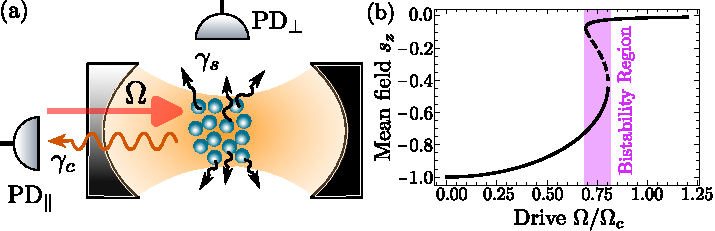
\includegraphics[width=0.8\textwidth]{img_1/fig_for_cavity.pdf}
        \caption{(a) System under study (b) Mean-field solution and bistability region}
    \end{figure}

    Main equation -- Master equation
    \begin{equation}
        \dot{\rho} = -i[{\cal H}, \rho] + \frac{\gamma_c}{2}{\cal D}[\hat{S}_-]\rho + \frac{\gamma_s}{2}\sum_n{\cal D}[\hat{\sigma}_n]\rho,\qquad {\cal H} = 2\Omega \hat{S}_x
    \end{equation}
\hfill{\scriptsize \underline{Leppenen}, Shahmoon, Phys. Rev. A 2026}
\end{frame}
\begin{frame}
    \frametitle{How to solve the master equation? Answer: MCWF method}

    Generally: Solve for density matrix: $4^N \times 4^N$ elements, $N$ is the number of qubits.\\
    Instead:
    Probabilistic unraveling of the master equation into quantum trajectories
    \begin{equation}
        \ket{\psi(t+dt)} = 
        \begin{cases}
            \frac{\hat{S}_-\ket{\psi(t)}}{\sqrt{p_-}} & \text{with probability } p_- = \gamma_c dt \langle \psi(t)|\hat{S}_+\hat{S}_-|\psi(t)\rangle \\
            \frac{\hat{\sigma}_n\ket{\psi(t)}}{\sqrt{p_n}} & \text{with probability } p_n = \gamma_s dt \langle \psi(t)|\hat{\sigma}_n^\dagger\hat{\sigma}_n|\psi(t)\rangle \\
            \frac{e^{-i{\cal H}_{NH}dt}\ket{\psi(t)}}{\sqrt{p_0}} & \text{with probability } p_0 = 1 - p_- - \sum_n p_n
        \end{cases}
    \end{equation}
    \cmark\ Saves memory: $2^N \times 2^N$ elements
    
    \xmark\ Loses Time: Need to average over many trajectories to get the density matrix.

    \vspace{1 cm}
    In our work we found that a bistability is seen in a single trajectory, but the bistability is lost in the density matrix average.
    \hfill{\scriptsize \underline{Leppenen}, Shahmoon, Phys. Rev. A 2026}
\end{frame}

\begin{frame}
    \frametitle{How typical trajectory looks like (in bistability case)}
    \begin{figure}
        \centering
        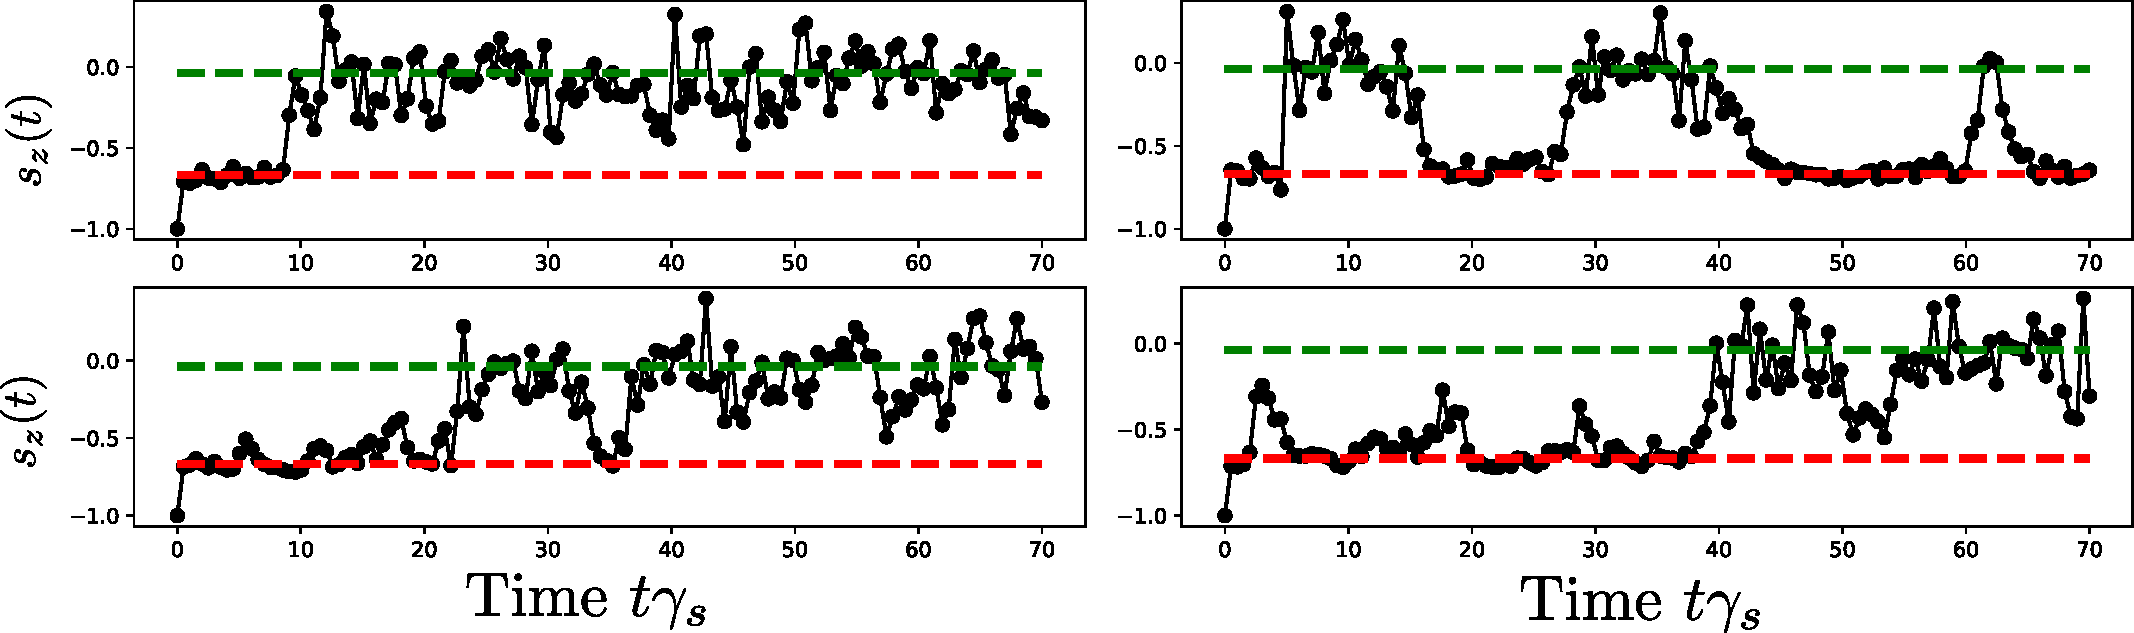
\includegraphics[width=\textwidth]{img_1/four_traj.pdf}
        \caption{4 examples of quantum trajectories $N = 18$ (best I can get), $\Omega = 0.73\Omega_c$ (bistability region), $\gamma_c = 10\gamma_s$. Red and Green lines are the mean-field solutions. Generated with QuTiP (python library for quantum simulations).}
    \end{figure}

    Note: average of $N_{tr} \approx 100$ trajectories gives the density matrix solution, which is a smooth curve (no bistability).
    \hfill{\scriptsize \underline{Leppenen}, Shahmoon, Phys. Rev. A 2026}
\end{frame}

\begin{frame}
    \frametitle{Problem statement}
      \begin{figure}
        \centering
        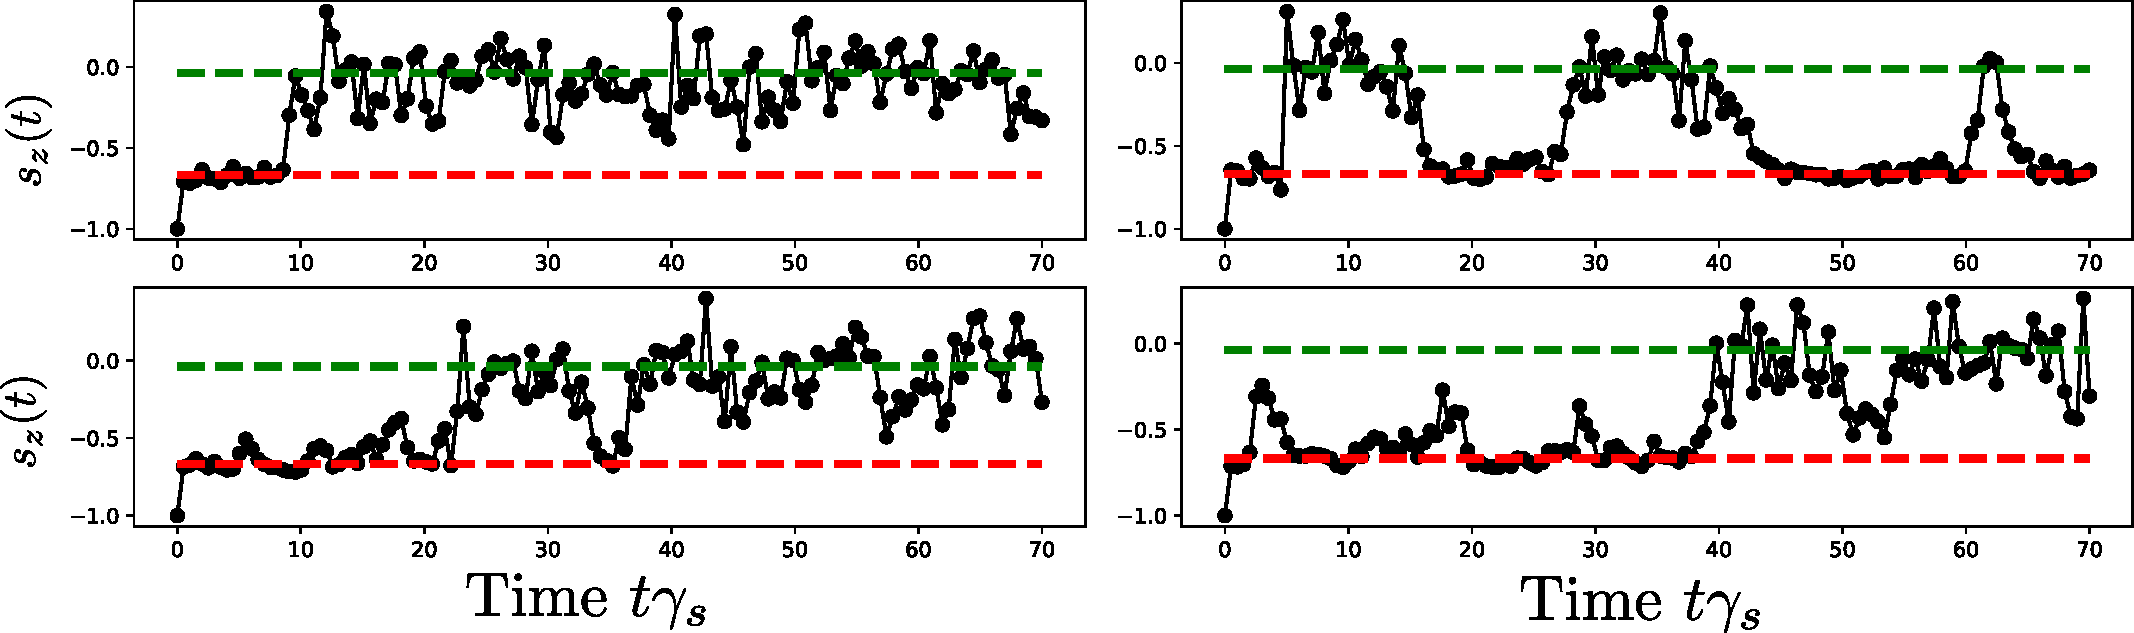
\includegraphics[width=\textwidth]{img_1/four_traj.pdf}
        \caption{4 examples of quantum trajectories $N = 18$ (best I can get), $\Omega = 0.73\Omega_c$ (bistability region), $\gamma_c = 10\gamma_s$.}
    \end{figure}  

    \vspace{-0.5cm}
    \begin{block}{Goal of the project}
        Create a model to generate trajectories similar to quantum trajectories generated by Monte Carlo wave-function simulations in QuTiP
    \end{block}
\end{frame}

\begin{frame}
    \frametitle{Why this matters?}

    \vspace{-1 cm}
    \begin{figure}
        \centering
        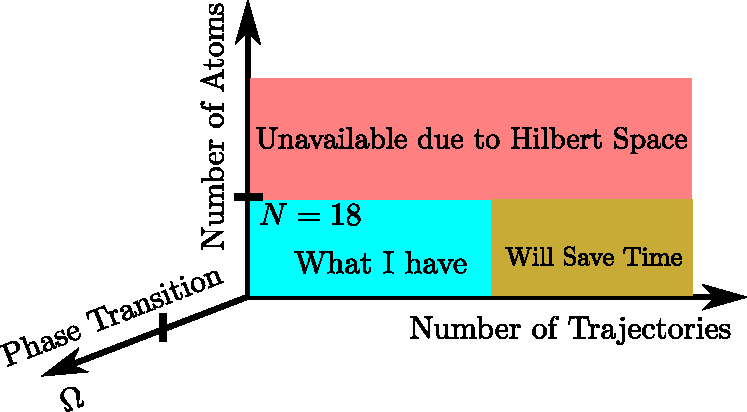
\includegraphics[width=0.6\textwidth]{img_1/logic1.pdf}
    \end{figure}
    \begin{block}{Directions}
      \begin{itemize}
        \item Fix $N$ and $\Omega$, generate more trajectories $\Rightarrow$ capture mean and/or bistability
        \item Fix $N$, generate trajectories for different $\Omega$ $\Rightarrow$ extrapolate to unseen $\Omega$ values
        \item Full model with $N$ and $\Omega$ 
      \end{itemize}
      
    \end{block}
\end{frame}


\section{Fixed $N$ and $\Omega$: Generating more trajectories}

\begin{frame}
    \tableofcontents
\end{frame}


\begin{frame}
    \frametitle{Dataset \& Model for $N = 8$}
    \begin{figure}
      \centering
      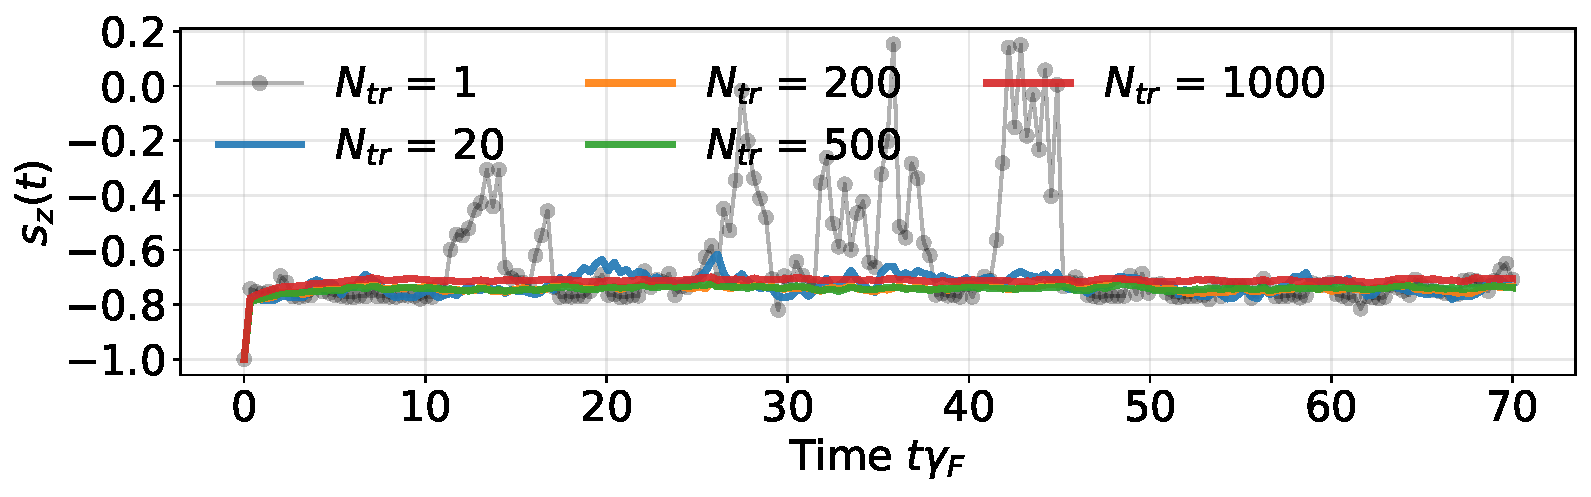
\includegraphics[width=0.8\textwidth]{img_1/example_N_8.pdf}
      \caption{Generated trajectory and averages for $N=8$ and $\Omega = 0.73\Omega_c$. Dataset contains $N_{tr} = 1000$ trajectories, each with $T=210$ time steps. We split it into training, testing and validation sets with ratio 80:10:10.}
    \end{figure}
    \begin{block}
      {We use a Gate Recurrent Unit (GRU) model for predicting time series on \textbf{discrete} grid}
      $x_{t+1} = f_{\theta}(x_t|h_t)$; $h_t$ -- \textit{hidden state}. Input: $x_t = [s_t, \tau_t]$; Output: $s_{t+1} \in [-1,1]$.
      \cmark
    \end{block}

    

\end{frame}


\begin{frame}{TrajectoryGRUGrid: Model Architecture}
\centering

\resizebox{\textwidth}{!}{%
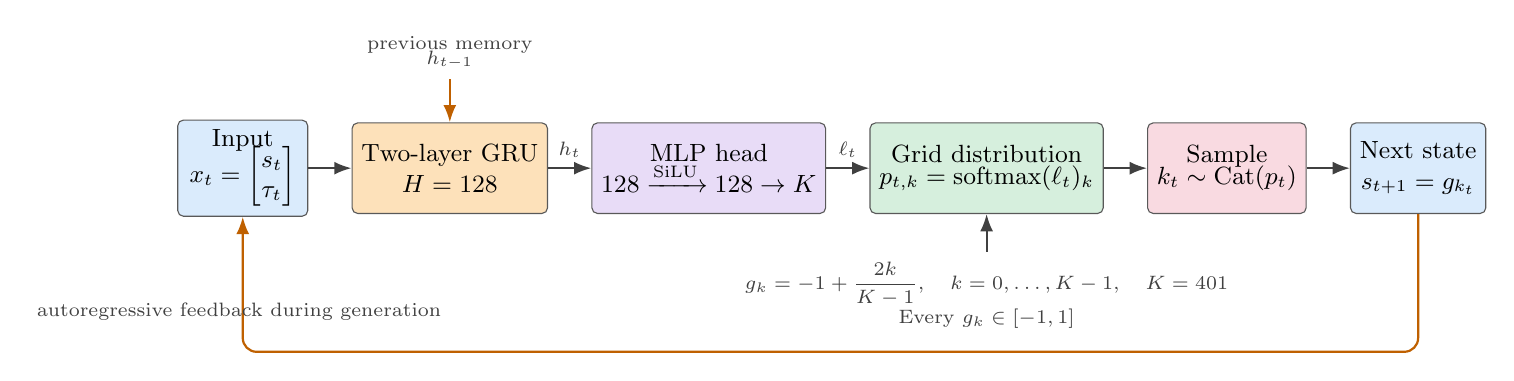
\begin{tikzpicture}[node distance=0.55cm]
  \node[
    modelnode,
    fill=inputblue,
    minimum width=1.65cm
  ] (input) {
    Input\\[-1mm]
    $\displaystyle x_t=
      \begin{bmatrix}s_t\\ \tau_t\end{bmatrix}$
  };

  \node[
    modelnode,
    fill=gruorange,
    minimum width=2.05cm,
    right=of input
  ] (gru) {
    Two-layer GRU\\
    $H=128$
  };

  \node[
    modelnode,
    fill=headpurple,
    minimum width=2.15cm,
    right=of gru
  ] (head) {
    MLP head\\
    $128\xrightarrow{\mathrm{SiLU}}128
      \rightarrow K$
  };

  \node[
    modelnode,
    fill=gridgreen,
    minimum width=1.85cm,
    right=of head
  ] (distribution) {
    Grid distribution\\[-1mm]
    $p_{t,k}=\operatorname{softmax}(\ell_t)_k$
  };

  \node[
    modelnode,
    fill=samplepink,
    minimum width=1.55cm,
    right=of distribution
  ] (sample) {
    Sample\\[-1mm]
    $k_t\sim\mathrm{Cat}(p_t)$
  };

  \node[
    modelnode,
    fill=inputblue,
    minimum width=1.35cm,
    right=of sample
  ] (nextstate) {
    Next state\\
    $s_{t+1}=g_{k_t}$
  };

  \draw[flow] (input) -- (gru);
  \draw[flow] (gru) -- node[above,annotation] {$h_t$} (head);
  \draw[flow] (head) -- node[above,annotation] {$\ell_t$} (distribution);
  \draw[flow] (distribution) -- (sample);
  \draw[flow] (sample) -- (nextstate);

  \node[annotation,above=0.55cm of gru] (previoushidden) {
    previous memory\\[-1mm]
    $h_{t-1}$
  };
  \draw[recurrent] (previoushidden.south) -- (gru.north);

  \node[annotation,below=0.48cm of distribution] (grid) {
    $\displaystyle
      g_k=-1+\frac{2k}{K-1},\quad
      k=0,\ldots,K-1,\quad K=401
    $\\
    Every $g_k\in[-1,1]$
  };
  \draw[flow] (grid.north) -- (distribution.south);

  \draw[recurrent,rounded corners=5pt]
    (nextstate.south)
    -- ++(0,-1.75)
    -| node[pos=0.72,below,annotation] {
      autoregressive feedback during generation
    }
    (input.south);
\end{tikzpicture}
}

\vspace{0.35cm}

\begin{block}{Training at every time step}
\small
\[
  y_t=s_{t+1}^{\mathrm{real}},
  \qquad
  q_{t,i}=1-\alpha,\quad q_{t,i+1}=\alpha,
  \qquad
  \mathcal{L}_t
  =-\sum_{k=0}^{K-1}q_{t,k}\log p_{t,k}.
\]
\vspace{-2mm}
\[
  \underbrace{\text{real }s_t\text{ as input}}_{\text{teacher forcing}}
  \quad\longrightarrow\quad
  \underbrace{\text{two-bin interpolated target }q_t}_{\text{continuous data on a discrete grid}}
  \quad\longrightarrow\quad
  \underbrace{\text{categorical cross-entropy}}_{\text{maximize next-state likelihood}} .
\]
\end{block}
\end{frame}

\end{document}